%=======================================================================
%  PRACTICA N.o 3 - SIMETRIA Y TRANSFORMACIONES DE SENALES EN PYTHON
%  Curso : Senales y Sistemas  (2026-2)
%  UCSP  - Facultad de Ingenieria - Ing. Electronica y de Telecomunicaciones
%  Docente     : (por confirmar)
%  Laboratorio : Ing. Jeanpier Ancori Sanchez
%
%  La guia NO procede de un .doc del docente: la escribe el autor sobre el
%  material que se dicto en la Semana 4 (Contenidos/Semana_4/), de donde salen
%  las funciones escalon, rampa y pulso y la descomposicion en parte par e
%  impar. Los nombres de las funciones son DELIBERADAMENTE los mismos que los
%  de los notebooks de clase: el alumno no tiene que traducir nada.
%
%  Version 1 - Practica de 45 minutos, sin hardware: se resuelve en Colab.
%
%  DURACION. El encargo es de 45 minutos de sesion, y eso manda sobre todo lo
%  demas. Se descarto el plan inicial de cinco ejercicios: con cinco enunciados
%  independientes el alumno repite cinco veces el mismo arranque (vector de
%  tiempo, plot, rotulado) y no llega al final. Quedan TRES ejercicios
%  encadenados, y el tercero opera sobre la senal que construyo el segundo, de
%  modo que la parte cara (dibujar bien) se paga una sola vez.
%
%  REPARTO DE TIEMPO. 10 + 20 + 15 minutos. El ejercicio 2 se lleva la mitad
%  porque es el unico donde el alumno escribe funciones desde cero (rampa y
%  pulso); escalon va dada en la plantilla para que el arranque no se coma la
%  sesion.
%
%  PUNTAJES. Suman 20 como exige el formato del curso, pero aqui los lleva cada
%  EJERCICIO (subseccion) y no la seccion IV: si el puntaje fuera al titulo de
%  la seccion y ademas a los ejercicios, la suma saldria doble. Reparto:
%  5 + 6 + 5 en el desarrollo, 2 el cuestionario y 2 las conclusiones.
%
%  LA SENAL DEL EJERCICIO 2. x(t) = r(t+2) - r(t) - 2u(t-1). Se eligio con tres
%  criterios: (1) que NO sea el trapecio del notebook 03, que esta resuelto ahi
%  mismo y se copiaria; (2) que obligue a la idea que mas cuesta, restar una
%  rampa para detener el crecimiento, en vez de sumar tramos sueltos; y (3) que
%  termine con una caida brusca, que solo se consigue con un escalon y no con
%  rampas. La figura objetivo va dibujada en la guia (figura 1) para que nadie
%  pierda tiempo interpretando el enunciado.
%
%  LA SENAL DEL EJERCICIO 1. x(t) = (t-1)^2, cuya descomposicion es exacta y
%  conocida de antemano: parte par t^2+1 y parte impar -2t. Asi la verificacion
%  numerica puede comparar contra el resultado teorico, no solo comprobar que
%  las dos partes suman la original. El notebook de clase usa t^2+t; se cambia
%  a proposito para que la respuesta no este ya escrita en el material.
%
%  VERIFICACION NUMERICA. Los tres ejercicios cierran con una celda que dice si
%  el resultado es correcto. Es lo que permite que 45 minutos alcancen: el
%  alumno no espera a la correccion para saber si le salio. De ahi tambien la
%  pregunta 3 del cuestionario, sobre por que se compara con np.allclose y no
%  con ==, que es el tropiezo clasico con numeros en coma flotante.
%
%  LO QUE NO ENTRA. Muestreo y aliasing, que estaban en el plan de cinco
%  ejercicios. Ya se vieron en el notebook 01 y no caben en 45 minutos junto a
%  simetria y transformaciones. Si en algun momento la sesion se amplia, ese es
%  el primer bloque que deberia volver.
%
%  SIN SECCION DE CONSTRUCCION. No hay montaje: el formato del curso la reserva
%  para el hardware, y la Practica 2 tampoco la lleva.
%
%  El preambulo se toma entero de Practica_2.tex para que las dos guias se vean
%  iguales. Se deja fuera circuitikz y pgfplots, que aqui no se usan: no hay
%  esquematicos y la unica figura es un PDF vectorial generado con matplotlib
%  por Codigo/generar_figura_objetivo.py.
%
%  Version 2 - Cinco ejercicios cortos, sin cuestionario ni conclusiones.
%
%  POR QUE. Lo pide el autor: cinco ejercicios, una o dos preguntas como mucho
%  y nada de cuestionario final. Se vuelve asi al plan de cinco que la version 1
%  habia descartado, pero sin caer en lo que lo hizo descartar: los ejercicios
%  NO son independientes. El 2 escribe rampa y pulso, el 3 las usa para armar
%  la senal, y el 4 y el 5 transforman esa misma senal. El arranque caro se
%  sigue pagando una sola vez; lo que cambia es que cada paso es mas corto.
%
%  COMO SE PARTIO. El antiguo ejercicio 2 (20 minutos: escribir las funciones Y
%  armar la senal) se divide en dos: el 2 solo escribe y prueba rampa y pulso,
%  el 3 solo arma la senal de la figura. El ejercicio 5 es nuevo: la
%  transformacion combinada x(-2t+1), que en la version 1 era la pregunta 2 del
%  cuestionario y ahora se hace en codigo en vez de contestarse en papel. Para
%  apuntalarlo entra en el marco teorico la subseccion de transformaciones
%  combinadas con un ejemplo resuelto (x(2t-4) sobre un pulso), que NO es el
%  caso del ejercicio.
%
%  PREGUNTAS. Quedan dos, dentro de los ejercicios 4 y 5, con sus lineas de
%  respuesta: cuanto dura x(2t) y entre que instantes vive x(-2t+1). Las otras
%  dos del cuestionario viejo (parte par de una senal impar, allclose frente a
%  ==) desaparecen; la nota tecnica sobre allclose se queda porque las celdas
%  de verificacion lo siguen usando.
%
%  PUNTAJES. 5 x 4 = 20. Al irse el cuestionario y las conclusiones, los 20
%  puntos los llevan enteros los ejercicios. Las secciones VI y VII del formato
%  del curso no aparecen: es decision del autor para esta practica, no un
%  olvido.
%
%  TIEMPOS. 8 + 8 + 12 + 9 + 8 = 45 minutos. Muestreo y aliasing siguen fuera,
%  por lo mismo que en la version 1.
%=======================================================================

\documentclass[11pt,a4paper]{article}

%------------------------------------------------------------- idioma
% Compilar con XeLaTeX (no con pdflatex): Trebuchet MS es una fuente TrueType
% del sistema y solo fontspec, bajo XeLaTeX o LuaLaTeX, sabe cargarla.
% inputenc y fontenc se omiten a proposito: XeLaTeX trabaja en UTF-8 de forma
% nativa y esos paquetes dan error con este motor.
\usepackage{fontspec}
\setmainfont{Trebuchet MS}[
  Path            = C:/Windows/Fonts/,
  Extension       = .ttf,
  UprightFont     = trebuc,
  BoldFont        = trebucbd,
  ItalicFont      = trebucit,
  BoldItalicFont  = trebucbi,
  Ligatures       = TeX
]
\usepackage[spanish,es-nodecimaldot]{babel}
\usepackage{microtype}

%----------------------------------------------------------- geometria
\usepackage[left=2.4cm,right=2.4cm,top=3.1cm,bottom=2.6cm,headheight=30pt,
            footskip=1.2cm]{geometry}

%------------------------------------------------------------ graficos
\usepackage{graphicx}
\usepackage{float}
\usepackage{placeins}
\usepackage[font=small,labelfont=bf,labelsep=period]{caption}
\usepackage{subcaption}
\captionsetup{subrefformat=parens}
\graphicspath{{imagenes/}}

%-------------------------------------------------------------- tablas
\usepackage{array}
\usepackage{tabularx}
\usepackage{booktabs}

%----------------------------------------------------- matematicas / SI
\usepackage{amsmath,amssymb}
\usepackage{siunitx}
\sisetup{
  output-decimal-marker = {,},
  per-mode              = symbol,
  range-phrase          = { a },
  range-units           = single,
  mode                  = match,
  detect-weight         = true,
  detect-family         = true
}

%--------------------------------------------------------------- listas
\usepackage{enumitem}
\setlist[itemize]{itemsep=3pt,topsep=4pt,parsep=0pt}
\setlist[enumerate]{itemsep=8pt,topsep=4pt,parsep=0pt}

%--------------------------------------------------------------- cajas
\usepackage[most]{tcolorbox}
\usepackage{pgffor}

\newtcolorbox{notatec}[1]{enhanced,breakable,
  colback=blue!3!white, colframe=blue!55!black,
  fonttitle=\bfseries\small, title={Nota técnica --- #1},
  boxrule=0.6pt, arc=2pt, left=6pt,right=6pt,top=4pt,bottom=4pt}

\newtcolorbox{seguridad}[1]{enhanced,breakable,
  colback=red!3!white, colframe=red!60!black,
  fonttitle=\bfseries\small, title={Seguridad --- #1},
  boxrule=0.6pt, arc=2pt, left=6pt,right=6pt,top=4pt,bottom=4pt}

\newtcolorbox{ejemplo}[1]{enhanced,breakable,
  colback=green!3!white, colframe=green!45!black,
  fonttitle=\bfseries\small, title={Ejemplo resuelto --- #1},
  boxrule=0.6pt, arc=2pt, left=6pt,right=6pt,top=4pt,bottom=4pt}

%---------------------------------------------------------------- codigo
% Solo hace falta componer nombres de funcion y lineas sueltas de Python, no
% listados completos: la plantilla los trae ya escritos. Con \texttt basta, y
% asi no entra listings, que con fontspec pide configuracion aparte.
\newcommand{\py}[1]{\texttt{#1}}

%------------------------------------------------------------ comandos
% Lineas punteadas para respuestas del alumno: \lineasresp{n}
\newcommand{\lineasresp}[1]{%
  \par\vspace{6pt}%
  \foreach \i in {1,...,#1}{\noindent\rule{\linewidth}{0.4pt}\par\vspace{11pt}}%
}

% Puntaje al final del titulo de una seccion calificada.
\newcommand{\puntos}[1]{\normalfont\normalsize\textmd{(#1 puntos)}}

%----------------------------------------------------- compaginacion
\usepackage{needspace}
\usepackage{etoolbox}
\pretocmd{\section}{\needspace{5\baselineskip}}{}{}
\pretocmd{\subsection}{\needspace{4\baselineskip}}{}{}
\widowpenalty=10000
\clubpenalty=10000

%------------------------------------------------------------ espaciado
\setlength{\intextsep}{9pt}
\setlength{\abovecaptionskip}{6pt}
\AtBeginDocument{%
  \setlength{\abovedisplayskip}{7pt}%
  \setlength{\belowdisplayskip}{7pt}%
  \setlength{\abovedisplayshortskip}{4pt}%
  \setlength{\belowdisplayshortskip}{4pt}%
}

%---------------------------------------------------- encabezado / pie
\usepackage{fancyhdr}
\pagestyle{fancy}
\fancyhf{}
\fancyhead[L]{\footnotesize UCSP --- Facultad de Ingeniería\\
              Ing. Electrónica y de Telecomunicaciones}
\fancyhead[R]{\footnotesize 2026-2 Señales y Sistemas\\
              Jeanpier Ancori Sánchez}
\fancyfoot[L]{\footnotesize Práctica N.\textsuperscript{o} 3 --- Simetría y transformaciones de señales}
\fancyfoot[R]{\footnotesize Página \thepage\ de \pageref{LastPage}}
\renewcommand{\headrulewidth}{0.4pt}
\renewcommand{\footrulewidth}{0.4pt}
\usepackage{lastpage}

%------------------------------------------------------- numeracion
\renewcommand{\thesection}{\Roman{section}}
\renewcommand{\thesubsection}{\arabic{subsection}}
\renewcommand{\thesubsubsection}{\thesubsection.\arabic{subsubsection}}
\setcounter{secnumdepth}{3}

%-------------------------------------------------------- hiperenlaces
\usepackage[hidelinks,pdfusetitle]{hyperref}
\usepackage{xurl}
\hypersetup{
  pdftitle={Practica 3 - Simetria y transformaciones de senales en Python},
  pdfsubject={Senales y Sistemas - Guia de practicas},
  pdfauthor={Jeanpier Ancori Sanchez},
  pdfkeywords={senales y sistemas, Python, NumPy, Matplotlib, Colab, senal par,
               senal impar, escalon unitario, rampa, pulso rectangular,
               desplazamiento, escalado, reflexion}
}

% babel-spanish rotula las tablas como "Cuadro"; los originales dicen "Tabla".
\addto\captionsspanish{\renewcommand{\tablename}{Tabla}}

\begin{document}

%=======================================================================
%  CABECERA DE LA GUIA
%=======================================================================
\begingroup
\renewcommand{\tabularxcolumn}[1]{m{#1}}
\renewcommand{\arraystretch}{2.0}
\setlength{\tabcolsep}{12pt}
\noindent
\begin{tabularx}{\textwidth}{|>{\centering\arraybackslash}m{2.2cm}|>{\centering\arraybackslash}X|>{\centering\arraybackslash}m{3.0cm}|}
\hline
\rule{0pt}{2.1cm}{\fontsize{58}{58}\selectfont\bfseries 3}
    & \begin{minipage}[c]{\linewidth}\centering
          {\large\bfseries Guía de Prácticas}\\[7pt]
          {\Large\bfseries Simetría y Transformaciones\\ de Señales en Python}
      \end{minipage}
    & {\Large\bfseries Nota}\\
\hline
\multicolumn{3}{|l|}{\rule{0pt}{1.3cm}\large\textbf{Grupo:}~\rule{4.6cm}{0.4pt}%
    \hfill\large\textbf{Fecha:}~\rule{4.6cm}{0.4pt}\hspace{2mm}}\\
\hline
\multicolumn{3}{|l|}{\rule{0pt}{1.2cm}\large\textbf{Alumno(s):}~\rule{11.2cm}{0.4pt}\hspace{2mm}}\\
\multicolumn{3}{|l|}{\rule{0pt}{1.2cm}\phantom{\large\textbf{Alumno(s):}}~\rule{11.2cm}{0.4pt}\hspace{2mm}}\\
\hline
\end{tabularx}
\endgroup

\vspace{0.8cm}

%=======================================================================
\section{Objetivos}
%=======================================================================
El objetivo de esta práctica es construir y manipular señales en Python con las
herramientas vistas en clase. Para ello se desarrollan las siguientes actividades:

\begin{itemize}
    \item Descomponer una señal cualquiera en su parte par y su parte impar, y
          comprobar numéricamente que la descomposición es correcta.
    \item Construir una señal definida por tramos combinando escalones, rampas y
          pulsos, en lugar de describirla trozo a trozo.
    \item Aplicar a esa señal el desplazamiento, la reflexión y el escalado de la
          variable independiente, primero por separado y después combinados.
    \item Presentar cada resultado en una figura rotulada, con título, ejes con
          unidades, rejilla y leyenda.
\end{itemize}

\FloatBarrier
%=======================================================================
\section{Marco teórico}
%=======================================================================

\subsection{Parte par y parte impar}
Una señal es \textbf{par} cuando $x(t) = x(-t)$, es decir cuando el eje vertical actúa
como un espejo; y es \textbf{impar} cuando $x(t) = -x(-t)$, de modo que al reflejarla
queda del revés. El coseno es par y el seno es impar.

La mayoría de las señales no son ni una cosa ni la otra, pero \textbf{cualquier señal se
puede escribir como la suma de una parte par y una parte impar}:

\begin{align}
  x_p(t) &= \frac{x(t) + x(-t)}{2} \label{eq:par}\\[4pt]
  x_i(t) &= \frac{x(t) - x(-t)}{2} \label{eq:impar}
\end{align}

\noindent y se cumple siempre que $x(t) = x_p(t) + x_i(t)$. En Python, $x(-t)$ se obtiene
llamando a la misma función con el vector de tiempo cambiado de signo.

\subsection{Funciones singulares}
El \textbf{escalón unitario} $u(t)$ vale \num{0} antes del origen y \num{1} a partir de
él. Es la pieza con la que se construye todo lo demás: sirve para \emph{encender} un
trozo de señal en un instante concreto.

A partir de él se definen la \textbf{rampa}, que crece con pendiente constante desde el
instante en que arranca, y el \textbf{pulso rectangular}, que no es más que la diferencia
de dos escalones:

\begin{align}
  r(t) &= t\,u(t) \\
  p(t) &= u(t-a) - u(t-b) \qquad \text{(pulso entre $a$ y $b$)}
\end{align}

Desplazando, escalando y restando estas tres piezas se arma cualquier señal definida por
tramos. La idea que más cuesta, y que se practica en el ejercicio~3, es que
\textbf{para detener un crecimiento hay que restar otra rampa}: una rampa, una vez que
arranca, ya no se para sola.

\subsection{Transformaciones de la variable independiente}
Las tres transformaciones actúan sobre el \emph{tiempo}, no sobre la amplitud:

\begin{itemize}
    \item \textbf{Desplazamiento:} $x(t - t_0)$ retrasa la señal $t_0$ segundos; con
          $x(t + t_0)$ se adelanta.
    \item \textbf{Reflexión:} $x(-t)$ la voltea respecto del eje vertical.
    \item \textbf{Escalado:} $x(at)$ con $a > 1$ la comprime, y con $0 < a < 1$ la
          expande. La duración queda dividida entre $a$.
\end{itemize}

\subsection{Transformaciones combinadas}
Cuando las tres aparecen a la vez, como en $x(at + b)$, en Python no hay que decidir
ningún orden: basta con \textbf{evaluar la función en el tiempo transformado}, por
ejemplo \py{x(a*t + b)}. Para saber \emph{dónde} queda la señal se plantea que el
argumento recorra el intervalo en el que la original es distinta de cero, y se despeja
$t$.

\begin{ejemplo}{dónde queda $p(2t-4)$}
Sea $p(t)$ un pulso entre $t = 0$ y $t = \qty{2}{\second}$. La señal $y(t) = p(2t - 4)$
es distinta de cero cuando su argumento cae dentro del pulso:
\begin{equation*}
  0 < 2t - 4 < 2 \quad\Longrightarrow\quad 4 < 2t < 6 \quad\Longrightarrow\quad 2 < t < 3
\end{equation*}
El pulso queda entre \qty{2}{\second} y \qty{3}{\second}: dura \qty{1}{\second}, la mitad
que el original, porque $a = 2$ lo comprime. En Python se dibuja con
\py{pulso(2*t - 4, 0, 2)}. Si $a$ es negativo, al dividir la desigualdad entre $a$
\textbf{se invierten los signos} $<$: esa inversión es la reflexión.
\end{ejemplo}

\begin{notatec}{comparar números en coma flotante}
Los resultados de \py{numpy} son números en coma flotante, y dos cálculos que en papel
dan lo mismo pueden diferir en el decimoquinto decimal. Por eso las comprobaciones de
esta práctica se escriben con \py{np.allclose(a, b)}, que pregunta si dos arreglos son
\emph{casi} iguales, y nunca con \py{a == b}, que compara elemento a elemento y exige
igualdad exacta.
\end{notatec}

\FloatBarrier
%=======================================================================
\section{Materiales}
%=======================================================================
\begin{itemize}
    \item 01 computadora con acceso a internet y una cuenta de Google para usar
          \emph{Google Colab}. No hay que instalar nada: \py{numpy} y \py{matplotlib}
          ya vienen incluidos.
    \item 01 plantilla \py{plantilla\_practica\_3.ipynb}, que se entrega con la guía y
          trae los \py{import}, la función \py{escalon} y las celdas ya rotuladas.
    \item Los tres notebooks de la Semana 4 como material de consulta. Se pueden tener
          abiertos durante la práctica.
\end{itemize}

\FloatBarrier
%=======================================================================
\section{Desarrollo}
%=======================================================================
La sesión dura \qty{45}{\minute}. Trabaje sobre la plantilla y respete el reparto de
tiempo de la tabla~\ref{tab:tiempos}: los ejercicios están encadenados. El~3 usa las
funciones que se escriben en el~2, y el~4 y el~5 transforman la señal que construye
el~3.

\begin{table}[H]
  \centering
  \caption[Reparto de la sesión]{Reparto de la sesión. Cada ejercicio vale \num{4} puntos; los
  cinco suman \num{20}.}
  \label{tab:tiempos}
  \small
  \begin{tabularx}{0.9\linewidth}{@{}>{\centering\arraybackslash}m{1.6cm}X>{\centering\arraybackslash}m{2.1cm}>{\centering\arraybackslash}m{1.9cm}@{}}
    \toprule
    \textbf{Ejercicio} & \textbf{Qué se hace} & \textbf{Tiempo} & \textbf{Puntos} \\
    \midrule
    1 & Descomponer una señal en parte par e impar & \qty{8}{\minute}  & 4 \\
    2 & Escribir y probar la rampa y el pulso      & \qty{8}{\minute}  & 4 \\
    3 & Construir una señal por tramos             & \qty{12}{\minute} & 4 \\
    4 & Desplazar, reflejar y escalar esa señal    & \qty{9}{\minute}  & 4 \\
    5 & Aplicarle una transformación combinada     & \qty{8}{\minute}  & 4 \\
    \bottomrule
  \end{tabularx}
\end{table}

\begin{notatec}{qué se exige de cada figura}
Toda figura de esta práctica debe llevar \textbf{título}, \textbf{ejes rotulados con sus
unidades}, \textbf{rejilla} y \textbf{leyenda} cuando haya más de una curva. Es la misma
regla que siguen los notebooks de clase. Una figura correcta pero sin rotular no recibe
el puntaje completo.
\end{notatec}

\noindent\textbf{Entrega.} Al terminar la sesión suba el notebook \textbf{ejecutado}, con
sus figuras visibles y las celdas de verificación impresas.

\subsection{Ejercicio 1: parte par y parte impar \puntos{4}}
Considere la señal
\begin{equation}
  x(t) = (t-1)^2, \qquad -4 \le t \le 4
\end{equation}

\begin{enumerate}[label=\textbf{\alph*)}, leftmargin=*, labelsep=0.6em]
    \item Escriba la función \py{senal(t)} que la devuelve y calcule su parte par y su
          parte impar con las ecuaciones~\eqref{eq:par} y~\eqref{eq:impar}. Recuerde que
          $x(-t)$ se obtiene llamando a \py{senal} con el tiempo cambiado de signo.
    \item Dibuje las tres señales en una figura de tres subgráficas, una debajo de otra.
    \item Desarrolle $(t-1)^2$ en papel, escriba en la celda de verificación la parte par
          y la parte impar que le salgan, y compruebe con \py{np.allclose} que coinciden
          con las calculadas.
\end{enumerate}

\needspace{11\baselineskip}
\subsection{Ejercicio 2: la rampa y el pulso \puntos{4}}
\begin{enumerate}[label=\textbf{\alph*)}, leftmargin=*, labelsep=0.6em]
    \item Escriba las funciones \py{rampa(t, pendiente, inicio)} y \py{pulso(t, a, b)}
          a partir de la función \py{escalon(t)} que trae la plantilla.
    \item Dibuje en una figura de tres subgráficas el escalón $u(t-1)$, una rampa de
          pendiente \num{2} que arranca en $t = \qty{-1}{\second}$ y un pulso entre
          $t = \qty{-1}{\second}$ y $t = \qty{2}{\second}$.
    \item Ejecute la celda de verificación: comprueba sus dos funciones en tres
          instantes cada una.
\end{enumerate}

\subsection{Ejercicio 3: construir una señal por tramos \puntos{4}}
La figura~\ref{fig:objetivo} muestra la señal $x(t)$ que debe construir. Sube con
pendiente \num{1} desde $t = \qty{-2}{\second}$, se estabiliza en \qty{2}{\volt} al
llegar a $t = 0$ y cae a cero de golpe en $t = \qty{1}{\second}$.

\begin{figure}[H]
  \centering
  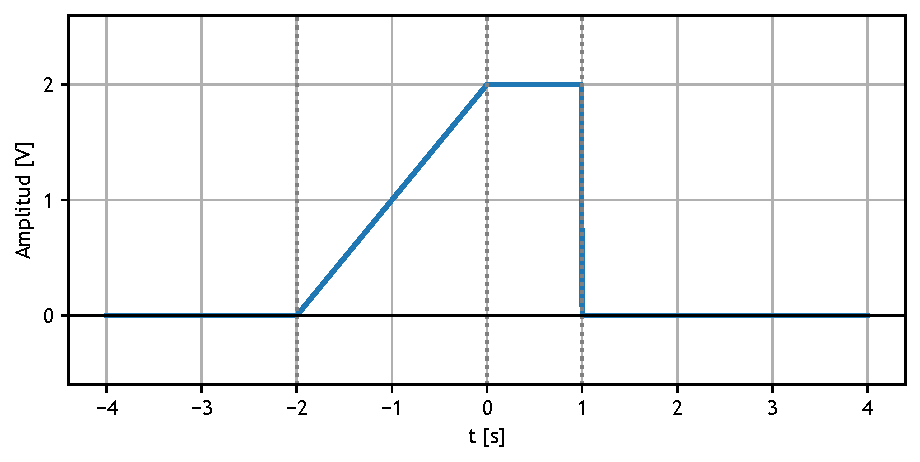
\includegraphics[width=0.78\linewidth]{senal_objetivo.pdf}
  \caption[Señal objetivo del ejercicio 3]{Señal objetivo del ejercicio~3. Las líneas
  punteadas marcan los tres instantes en los que cambia su comportamiento:
  $t = \qty{-2}{\second}$, $t = 0$ y $t = \qty{1}{\second}$.}
  \label{fig:objetivo}
\end{figure}

\begin{enumerate}[label=\textbf{\alph*)}, leftmargin=*, labelsep=0.6em]
    \item Construya la señal en la función \py{x\_tramos(t)} combinando las funciones del
          ejercicio~2. \textbf{No la defina tramo a tramo}: debe salir de sumar y restar
          rampas y escalones. Tenga presente que una rampa, una vez que arranca, sigue
          creciendo para siempre: para dejarla plana hay que restarle otra.
    \item Dibújela sobre el mismo intervalo de la figura y ejecute la celda de
          verificación: la señal debe valer \num{0} en $t = \qty{-3}{\second}$, \num{1}
          en $t = \qty{-1}{\second}$, \num{2} en $t = \qty{0.5}{\second}$ y de nuevo
          \num{0} en $t = \qty{1.5}{\second}$.
\end{enumerate}

\subsection{Ejercicio 4: desplazar, reflejar y escalar \puntos{4}}
Sobre la señal del ejercicio~3, dibuje en una figura de tres subgráficas, cada una junto
a $x(t)$ para poder compararlas:

\begin{enumerate}[label=\textbf{\alph*)}, leftmargin=*, labelsep=0.6em]
    \item $x(t-2)$
    \item $x(-t)$
    \item $x(2t)$
\end{enumerate}

\noindent Indique en el título de cada subgráfica qué transformación se aplicó.

\par\medskip
\needspace{6\baselineskip}
\noindent\textbf{Pregunta.} La señal original es distinta de cero entre
\qty{-2}{\second} y \qty{1}{\second}, es decir durante \qty{3}{\second}. ¿Entre qué
instantes lo es $x(2t)$, y cuánto dura?
\lineasresp{2}

\subsection{Ejercicio 5: una transformación combinada \puntos{4}}
\begin{enumerate}[label=\textbf{\alph*)}, leftmargin=*, labelsep=0.6em]
    \item Dibuje $y(t) = x(-2t + 1)$ junto a $x(t)$, en una sola gráfica con leyenda.
          Basta con evaluar \py{x\_tramos} en el tiempo transformado.
    \item Ejecute la celda de verificación, que comprueba $y(t)$ en cuatro instantes.
\end{enumerate}

\par\medskip
\needspace{6\baselineskip}
\noindent\textbf{Pregunta.} ¿Entre qué instantes es $y(t)$ distinta de cero? Obténgalo
despejando $t$, como en el ejemplo resuelto del marco teórico, y compruebe que coincide
con su gráfica.
\lineasresp{3}

\end{document}
